\documentclass[a4paper]{article}

\usepackage[english]{babel}
\usepackage[utf8]{inputenc}
\usepackage[T1]{fontenc}
\usepackage{amsmath}
\usepackage{graphicx}
\usepackage{listings}
\usepackage{color}
\usepackage{indentfirst}
\usepackage{hyperref}
\usepackage{float}
\usepackage{minted}
\usepackage{mathtools}

% Mniejsze marginesy
\addtolength{\textwidth}{3cm}
\addtolength{\hoffset}{-1.5cm}
\addtolength{\textheight}{3cm}
\addtolength{\voffset}{-1.5cm}


% START STRONY PIERWSZEJ


% Odstęp po akapicie
\setlength{\parskip}{1ex plus 0.5ex minus 0.5ex}

\begin{document}

\begin{titlepage}

\newcommand{\HRule}{\rule{\linewidth}{0.5mm}}

\center % Center everything on the page


\textsc{\large Politechnika Wrocławska}\\[4cm]


\HRule \\[0.6cm]
{\huge \bfseries Układy Cyfrowe i Systemy Wbudowane 2}\\[0.4cm]
\textsc{\Large projekt - Gra z wykorzystaniem myszy PS/2}\\[0.4cm]
\HRule \\[0.5cm]

{\textsc{\large termin zajęć: wtorek TP 11:00}}\\[1.0cm]

\begin{minipage}{0.4\textwidth}
	\begin{flushleft} \large
		\emph{Autorzy:}\\[0.1cm]
      XXXX
	\end{flushleft}
\end{minipage}
~
\begin{minipage}{0.5\textwidth}
	\begin{flushright} \large
		\emph{Prowadzący:} \\[0.1cm]
    XXXX
	\end{flushright}
\end{minipage}\\[1cm]

\vfill

{\large Wrocław 2018}

\end{titlepage}




% STRONA 2 - SPIS TREŚCI

\tableofcontents
\newpage






% STRONA 3 - WŁASCIWY START DOKUMENTU

%%%%%%%%%%%%%%%%%%%%%%%%%%%%%%%%%%%%%%%%%%%%%%%%%%%%%%%%%%%%%%%%%%%%%%%%%%%%%%%%%%%%%%%%%%%%%%%%%%%%%%%%%%%%%%%%%%%%%%%
\section{Wprowadzenie}
%%%%%%%%%%%%%%%%%%%%%%%%%%%%%%%%%%%%%%%%%%%%%%%%%%%%%%%%%%%%%%%%%%%%%%%%%%%%%%%%%%%%%%%%%%%%%%%%
\subsection{Cel i zakres projektu}

Głównym celem projektu było stworzenie zaimplementowanie w układzie cyfrowym gry, gdzie wyświetlanie grafiki odbywało by się poprzez złącze VGA, a sterowanie w grze poprzez PS/2\_Mouse. Głównym zadaniem gracza jest wydostanie się z labiryntu przedstawionego na ekranie poprzez kierowanie kursorem myszy nie dotykając ścian tego labiryntu. Gracz przegrywa gdy dotknie ściany, a wygrywa gdy dotknie górnej krawędzi ekranu.

Etapy prac nad projektem w ciągu semestru prezentowały się następująco:

\begin{itemize}

	\item Wyświetlanie obrazu na monitorze VGA oraz jego konfiguracja do częstotliwości 72Hz w rozdzielczości 800x600
    
    \item Implementacja obsługi myszki PS/2.
    
	\item Organizacja pamięci ROM i wyrysowanie dzięki niej planszy na ekranie.
    
    \item Poprawki i testowanie

\end{itemize}

%%%%%%%%%%%%%%%%%%%%%%%%%%%%%%%%%%%%%%%%%%%%%%%%%%%%%%%%%%%%%%%%%%%%%%%%%%%%%%%%%%%%%%%%%%%%%%%%
\subsection{Opis Sprzętu}

W naszym projekcie korzystaliśmy z platformy sprzętowej zestawu "S3EStarter Kit" firmy Digilent, monitora VGA i myszki PS/2. Co do samego układu to jego dokładny opis oraz specyfikacja znajdują się w dokumentacji. Warto jednak wspomnieć o samej specyfikacji Xilinx xc3s500e która prezentuje się następująco na tle jego bliźniaczych płytek:

\begin{figure}[h]
  \caption{Specyfikacja xc3s500e}
  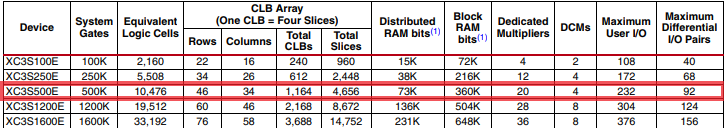
\includegraphics[scale=0.7]{xc3s500e.png}
  \centering
\end{figure}

\begin{figure}[h]
  \caption{Wygląd płyty układu cyfrowego XC3S500e}
  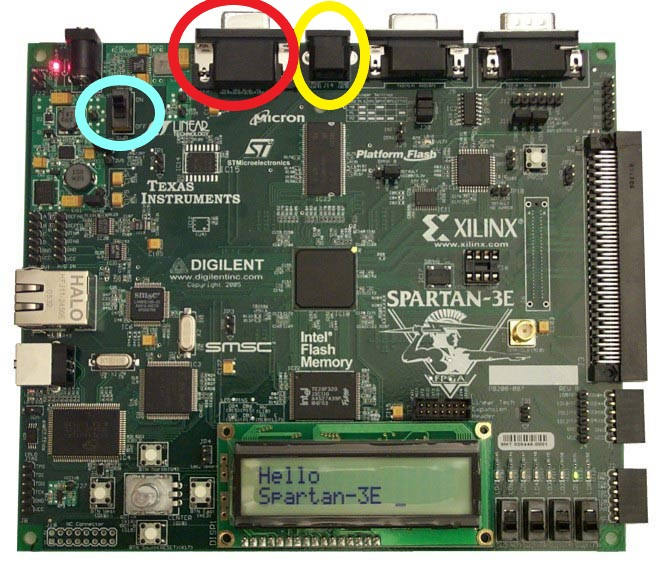
\includegraphics[scale=0.35]{plyta}
  \centering
\end{figure}

Oznaczenia:
\begin{itemize}
\item \textcolor{cyan}{jasnoniebieski} - włącznik płytki
\item \textcolor{red}{czerwony} - złącze VGA
\item \textcolor{yellow}{żółty} - wejście PS/2
\end{itemize}


\newpage

%%%%%%%%%%%%%%%%%%%%%%%%%%%%%%%%%%%%%%%%%%%%%%%%%%%%%%%%%%%%%%%%%%%%%%%%%%%%%%%%%%%%%%%%%%%%%%%%
\subsection{Zagadnienia teoretyczne (interfejsy, protokoły)}

W naszym projekcie, wykorzystaliśmy następujące interfejsy:
\begin{itemize}

  \item VGA - odpowiada za wyświetlanie sygnału na monitorze CRT

\end{itemize}

Użyliśmy również następujących protokołów ze strony kursu:

\begin{itemize}

  \item PS/2\_Mouse - moduł odpowiedzialny za obsługę myszki

\end{itemize}




%%%%%%%%%%%%%%%%%%%%%%%%%%%%%%%%%%%%%%%%%%%%%%%%%%%%%%%%%%%%%%%%%%%%%%%%%%%%%%%%%%%%%%%%%%%%%%%%%%%%%%%%%%%%%%%%%%%%%%%
\section{Projekt}
%%%%%%%%%%%%%%%%%%%%%%%%%%%%%%%%%%%%%%%%%%%%%%%%%%%%%%%%%%%%%%%%%%%%%%%%%%%%%%%%%%%%%%%%%%%%%%%%
\subsection{Schemat projektu}


\begin{figure}[h]
  \caption{Schemat projektu}
  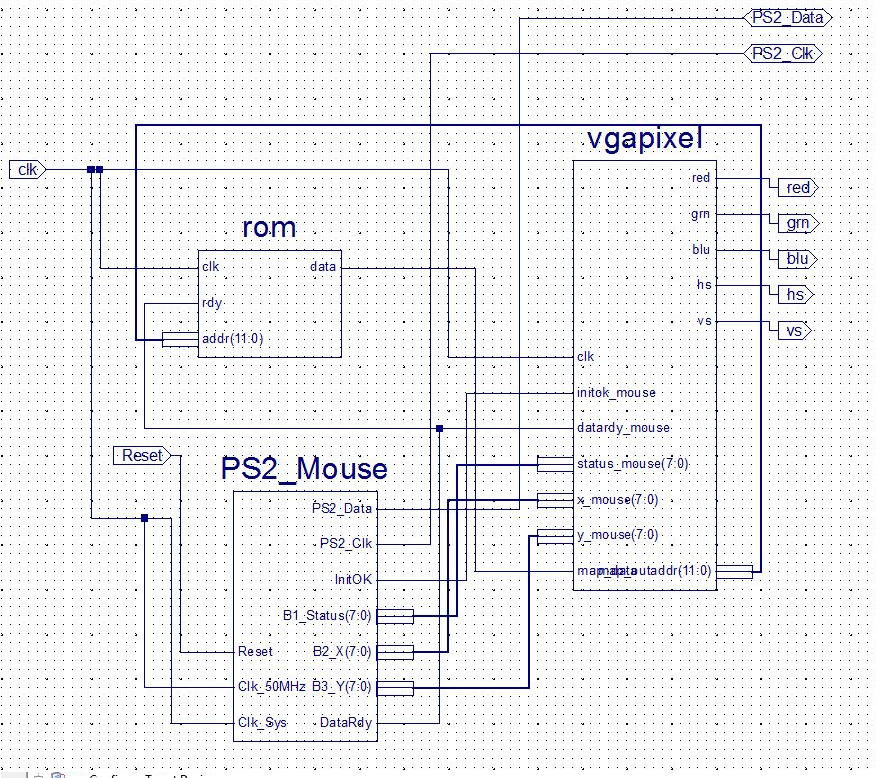
\includegraphics[scale=0.65]{schemat}
  \centering
\end{figure}

Powyższy rysunek przedstawia schemat naszego projektu, widzimy na nim wszystkie używane przez nas moduły: gotowe ze strony kursu oraz zaimplementowane przez nas. Głównym modułem naszego projektu jest $vgapixel$, który steruje monitorem, mający za zadanie wyświetlać obraz w dobrej częstotliwości oraz rozdzielczości, ponadto wyrysowuje ramkę na czterech brzegach naszego ekranu, co umożliwia zarówno łatwo zauważenie granic ekranu gry, jak i daje możliwość wygrania poprzez dotknięcie górnej krawędzi. $PS\_2Mouse$ obsługuję myszkę, natomiast $rom$ przechowuje obraz labiryntu w postaci ciągu zer i jedynek, każda jedynka jest jednym kwadratem z 2367 z których składa się nasz ekran. Dzięki temu ciągowi nasz $vgapixel$ jest w stanie wyrysować na ekranie labirynt, np w kolorze czerwonym. 

\subsection{Hierarchia i schemat}

\begin{figure}[h]
  \caption{Hierarchia projektu}
  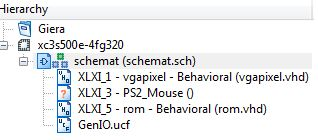
\includegraphics[scale=1.0]{hierarchia}
  \centering
\end{figure}
%%%%%%%%%%%%%%%%%%%%%%%%%%%%%%%%%%%%%%%%%%%%%%%%%%%%%%%%%%%%%%%%%%%%%%%%%%%%%%%%%%%%%%%%%%%%%%%%
\subsection{Moduły}

%%%%%%%%%%%%%%%%%%%%%%%%%%%%%%%%%%%%%%%%%%%%%%%%%%%%%%%%%%%%%%%%%%%%%%%%%%%%
\subsubsection{Plik UCF}

W pliku $GenIO.ucf$ zawarte są informacje co do wejść jak i wyjść ukazanych na schemacie. Fragment pliku wymaganego do poprawnego działania projektu:\\

NET "clk" LOC = "C9" | IOSTANDARD = LVTTL | PERIOD = 20.0ns HIGH 50;\\
NET "reset" LOC = "K17" | IOSTANDARD = LVTTL | PULLDOWN;\\
NET "PS2\_Data" LOC = "G13" | IOSTANDARD = LVCMOS33 | SLEW = SLOW | DRIVE = 8;\\
NET "PS2\_Clk"  LOC = "G14" | IOSTANDARD = LVCMOS33 | SLEW = SLOW | DRIVE = 8;\\
NET "red"  LOC = "H14" | IOSTANDARD = LVTTL | SLEW = FAST | DRIVE = 8;\\
NET "grn"  LOC = "H15" | IOSTANDARD = LVTTL | SLEW = FAST | DRIVE = 8;\\
NET "blu"  LOC = "G15" | IOSTANDARD = LVTTL | SLEW = FAST | DRIVE = 8;\\
NET "hs" LOC = "F15" | IOSTANDARD = LVTTL | SLEW = FAST | DRIVE = 8;\\
NET "vs" LOC = "F14" | IOSTANDARD = LVTTL | SLEW = FAST | DRIVE = 8;\\


\subsubsection{PS/2\_Mouse}
\begin{itemize}
\item Sygnały wejściowe: $clk$, $Reset$
\item Sygnały wyjściowe: $PS2\_Data$, $PS2\_Clk$, $InitOk$, $B1\_Status$, $B2\_X$, $B3\_Y$, $DataRdy$
\end{itemize}

Moduł ten odbiera kody wysyłane przez mysz PS/2, które determinują różne zdarzenia wykonane przez myszkę np. naciśnięcie myszki czy jej poruszenie.

Jeżeli $Datardy = '1'$ to oznacza gotowość na odbiór informacji od myszki. Wtedy na wyjścia B1\_Status, B2\_X i B3\_Y wysyłane są kolejno 3 bajty: status myszki (np. który przycisk naciśnięty), przesunięcie w pionie jak i w poziomie.

Jeżeli moduł został dopiero uruchomiony należy zaczekać, aż sygnał INIT\_OK = ‘1’.

%%%%%%%%%%%%%%%%%%%%%%%%%%%%%%%%%%%%%%%%%%%%%%%%%%%%%%%%%%%%%%%%%%%%%%%%%%%%
\subsubsection{rom}
\begin{itemize}
\item Sygnały wejściowe: $clk$, $rdy$, $addr(11:0)$
\item Sygnały wyjściowe: $data$
\end{itemize}

Cały nasz kod w tym module jest dość mało skomplikowany, jego główną częścią jest mapa samego labiryntu, która jest łatwo modyfikowalna

\begin{minted}{vhdl}
architecture Behavioral of rom is
   type rom_block is array (0 to 37 * 64 - 1) of STD_LOGIC;
   signal ROM : rom_block:= 
\end{minted}
Po tej części następuję wyrysowanie mapy w następujący sposób:

\begin{figure}[H]
  \caption{Tablica z mapą labiryntu, pierwsze 21 linijek bloku}
  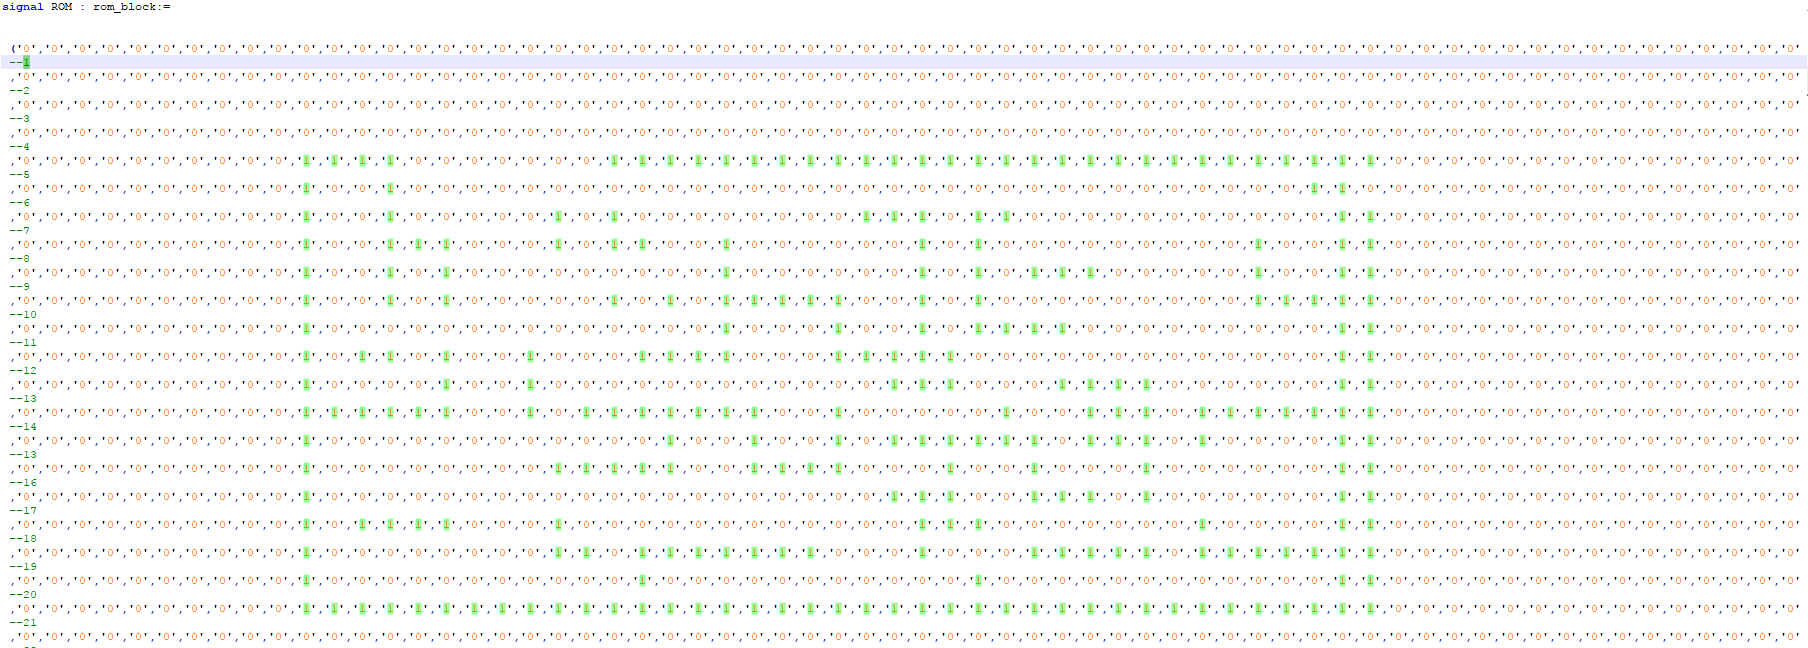
\includegraphics[width=15cm, height=8cm]{mapa}
  \centering
\end{figure}

Powyższe zdjęcie jest oczywiście jedynie istotną częścią naszego ekranu, na której znajduję się labirynt, jako iż na zdjęciu jest przedstawionych 21 linijek, pod nimi znajduję się dokładnie 15 z samymi zerami, które postanowiliśmy pominąć, aby obrazek był czytelny. 

Reszta kodu prezentuję się w następujący sposób:

\begin{minted}{vhdl}
begin
   process (clk)
   begin
        if (clk'event and clk = '1') then
            --if (rdy = '1') then
               data <= ROM(conv_integer(addr));
            --end if;
        end if;
   end process;
end Behavioral;
\end{minted}

Odpowiedzialna ona jest za przypisywanie do zmiennej data, która jest jedyną zmienną wyjściową, skonwertowanych wartości ROMU, za pomocą 12 bitowej tablicy addr. 12-bitowej, gdyż 
\begin{equation} (37 * 64 - 1) = 2367 \end{equation} 
mieści się na dwunastu bitach 
\begin{equation} 2^{12} = 4096\end{equation}


%%%%%%%%%%%%%%%%%%%%%%%%%%%%%%%%%%%%%%%%%%%%%%%%%%%%%%%%%%%%%%%%%%%%%%%%%%%%
\subsubsection{vgapixel}
\begin{itemize}
\item Sygnały wejściowe: $clk$, $initok\_mouse$, $datarrdy\_mouse$, $status\_mouse(7:0)$, $x\_mouse(7:0)$, $y\_mouse(7:0)$, $map\_data$
\item Sygnały wyjściowe: $red$, $grn$, $blu$, $hs$, $vs$, $map\_outaddr$
\end{itemize}

Sygnał $Clk$ jest używany praktycznie przez każdy proces, pozwala on na synchronizację między procesami.

Poniższy kawałek kodu odpowiada za zamianę wartości liczników poziomych i pionowych, które przechowują aktualnie sprawdzaną pozycję na ekranie na sygnał wyjściowy $map\_outaddr$, zawarta tu jest aktualnie sprawdzana pozycja. Otrzymujemy wtedy informację czy w pamięci znajduje się w tym miejscu ściana labiryntu:
\begin{minted}{vhdl}
   addrroundx <= std_logic_vector(to_unsigned(horz_counter, 10)(9 downto 4));
   addrroundy <= std_logic_vector(to_unsigned(vert_counter, 10)(9 downto 4));
   map_outaddr <= addrroundy & addrroundx;
\end{minted}

Część kodu odpowiedzialna za obsługę ruchu myszki. Przyjmowane są tu sygnały $x\_mouse$ i $y\_mouse$ które pozwalają obliczyć przesunięcie (offset) od ostatnio pamiętanej pozycji myszki. Jeżeli mysz jest aktywna i wykryte zostanie przesunięcie, kursor myszy zostanie ustawiony z nową pozycją. Jest tu też sprawdzane, czy gracz nie próbuje wyjść kursorem poza ekran, jeżeli tak to pozycja nie ustawi się poza ustalony obszar:
\begin{minted}{vhdl}
   moveMouse : process (clk, x_mouse, y_mouse, datardy_mouse)
   begin
      offsetX <= to_integer(signed(x_mouse));
      offsetY <= to_integer(signed(y_mouse));
      if rising_edge( clk ) AND datardy_mouse = '1' then 
         if (x_position + offsetX) > leftboundScreen + cursorSize / 2 AND (x_position + offsetX) < rightboundScreen - cursorSize / 2 then 
            x_position <= x_position + offsetX;
         end if;
         if (y_position - offsetY) > upboundScreen + cursorSize / 2 AND (y_position - offsetY) < downboundScreen - cursorSize / 2 then 
            y_position <= y_position - offsetY;
         end if;
      end if;
   end process moveMouse; 
\end{minted}

Wszystkie poniższe fragmenty kodu, aż do wyrysowania granic ekranu stanowią część procesu showGraphics, który przyjmuję $clk$, oraz $map_data$.

Na samym początku następuje czyszczenie ekranu poprzez podanie koloru ekranu czyli czarnego w standardzie RGB jest to (0,0,0):
\begin{minted}{vhdl}
      -- czyszczenie ekranu
      blu <= '0';
      grn <= '0';
      red <= '0';
  \end{minted}

Część kodu odpowiedzialna za wyrysowanie labiryntu, według mapy jaką ustalimy za pomocą 0 i 1 w module $rom$. W tym miejscu znana jest już dla danej pozycji czy powinna być tu ściana czy nie.
\begin{minted}{vhdl}
      if map_data = '1' then
         red <= '1';
         blu <= '0';
         grn <= '0';
 	  end if; 
\end{minted}

Fragment kodu odpowiedzialna za wykrywanie kolizji, jeśli ona nastąpi to flaga $lose$ ustawiona zostaje na '1'.
\begin{minted}{vhdl}
      -- jesli kolizja
      if map_data = '1' 
         and y_position + (cursorSize / 2) > vert_counter 
         and y_position - (cursorSize / 2) < vert_counter        
         and x_position + (cursorSize / 2) > horz_counter             
         and x_position - (cursorSize / 2) < horz_counter 
         then  
            lose <= '1';
      end if; 
\end{minted}

Gracz wygrywa, gdy dojedzie do górnej granicy ekranu, co obsługujemy tym fragmentem kodu:
\begin{minted}{vhdl}
      if y_position < 30 then
         win <= '1';
      end if;
\end{minted}


Segment kodu odpowiedzialny za rysowanie kursora myszki, który jest jednocześnie reprezentacja naszego gracza, myszka znika gdy gracz przegrał, natomiast gdy gracz wygra jego kursor staje się zielony:
\begin{minted}{vhdl}
      if vert_counter > y_position - (cursorSize / 2) 
         and vert_counter < y_position + (cursorSize / 2)
         and horz_counter > x_position - (cursorSize / 2)
         and horz_counter < x_position + (cursorSize / 2)
         and lose = '0' -- jesli przegrana to myszka zniknie
         then
         red <= '1';
         blu <= '1';
         grn <= '1';
         if win = '1' then 
            red <= '0';
            blu <= '0';
            grn <= '1';
         end if;
      end if;  
\end{minted}



Część kodu odpowiedzialna za wyrysowanie linii na wszystkich czterech granicach ekranu, z czego linia czerwona to ta, której należy dotknąć by wygrać:
\begin{minted}{vhdl}
      -- granice ekranu
      if vert_counter = upboundScreen then
         red <= '1';
      elsif vert_counter = downboundScreen then
         blu <= '1';
      elsif horz_counter = leftboundScreen then
         grn <= '1';
      elsif horz_counter = rightboundScreen then
         blu <= '1';
         grn <= '1';
      end if;
\end{minted}


\newpage

%%%%%%%%%%%%%%%%%%%%%%%%%%%%%%%%%%%%%%%%%%%%%%%%%%%%%%%%%%%%%%%%%%%%%%%%%%%%%%%%%%%%%%%%%%%%%%%%%%%%%%%%%%%%%%%%%%%%%%%
\section{Implementacja}
%%%%%%%%%%%%%%%%%%%%%%%%%%%%%%%%%%%%%%%%%%%%%%%%%%%%%%%%%%%%%%%%%%%%%%%%%%%%%%%%%%%%%%%%%%%%%%%%
\subsection{Rozmiar}
\begin{figure}[H]
  \caption{Raport projektu wygenerowany w Xilinx ISE}
  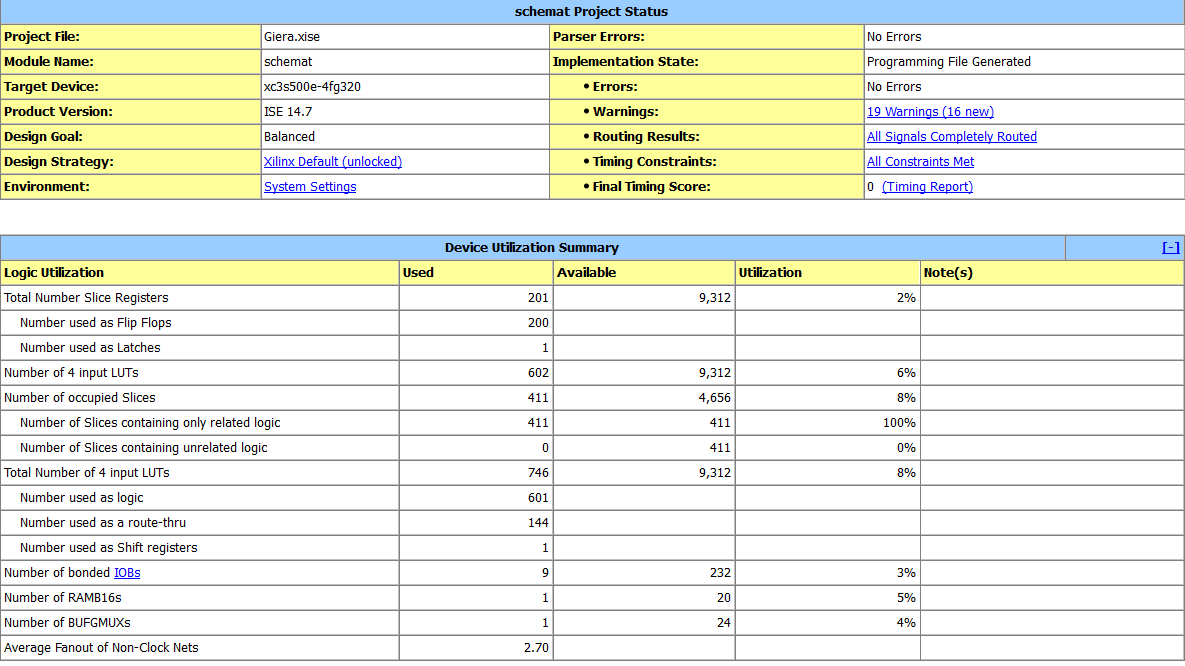
\includegraphics[scale=0.5]{statusProj}
  \centering
\end{figure}
W powyższym raporcie przedstawiono wybrane parametry naszego projektu. Wynika z niego, że używa jedynie 2\% dostępnych zasobów (slice registers). Użyta ilość tabel LUT to 6\% maksymalnej ilości, natomiast ilość zużytego RAMB16 to 5\%.

%%%%%%%%%%%%%%%%%%%%%%%%%%%%%%%%%%%%%%%%%%%%%%%%%%%%%%%%%%%%%%%%%%%%%%%%%%%%%%%%%%%%%%%%%%%%%%%%
\subsection{Szybkość}

\begin{figure}[H]
  \caption{ Raport dotyczący czasów wygenerowany w Xilinx ISE }
  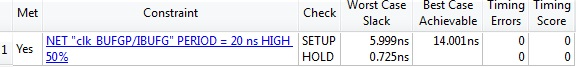
\includegraphics[scale=0.8]{memory}
  \centering
\end{figure}

Częstotliwość zegara w naszym projekcie wynosi 50 MHz czyli inaczej jeden cykl zegara trwa 20 ns. Raport przedstawia ograniczenia czasowe. Wynika z nich, że Worst Case Slack dla Setup wynosi 5,999 ns, a dla Hold 0,725 ns. Wartości dodatnie oznaczają iż ograniczenia są spełnione. Best Case Achievable - czyli najlepszy przypadek dostępności który jest dostępny tylko dla SETUP wynosi 14.001 ns. wynika z tego, że mieścimy się w jednym cyklu zegara, który jak wcześniej wspomnieliśmy trwa 20 ns. Prawdopodobnie nasz układ nie działałby gdybyśmy użyli 100 MHz. Sam raport nie wykazał żadnych błędów związanych z zegarem.


%%%%%%%%%%%%%%%%%%%%%%%%%%%%%%%%%%%%%%%%%%%%%%%%%%%%%%%%%%%%%%%%%%%%%%%%%%%%%%%%%%%%%%%%%%%%%%%%
\subsection{Podręcznik}

Przed uruchomieniem należy podłączyć do portu VGA na płytce monitor komputerowy o rozdzielczości 800x600, mysz PS/2 natomiast do portu PS/2. Należy wtedy uruchomić program $Impact$ i zaprogramować płytkę. Po uruchomieniu pokazuje nam się start gry przedstawiony poniżej.

\begin{figure}[H]
  \caption{Początek gry}
  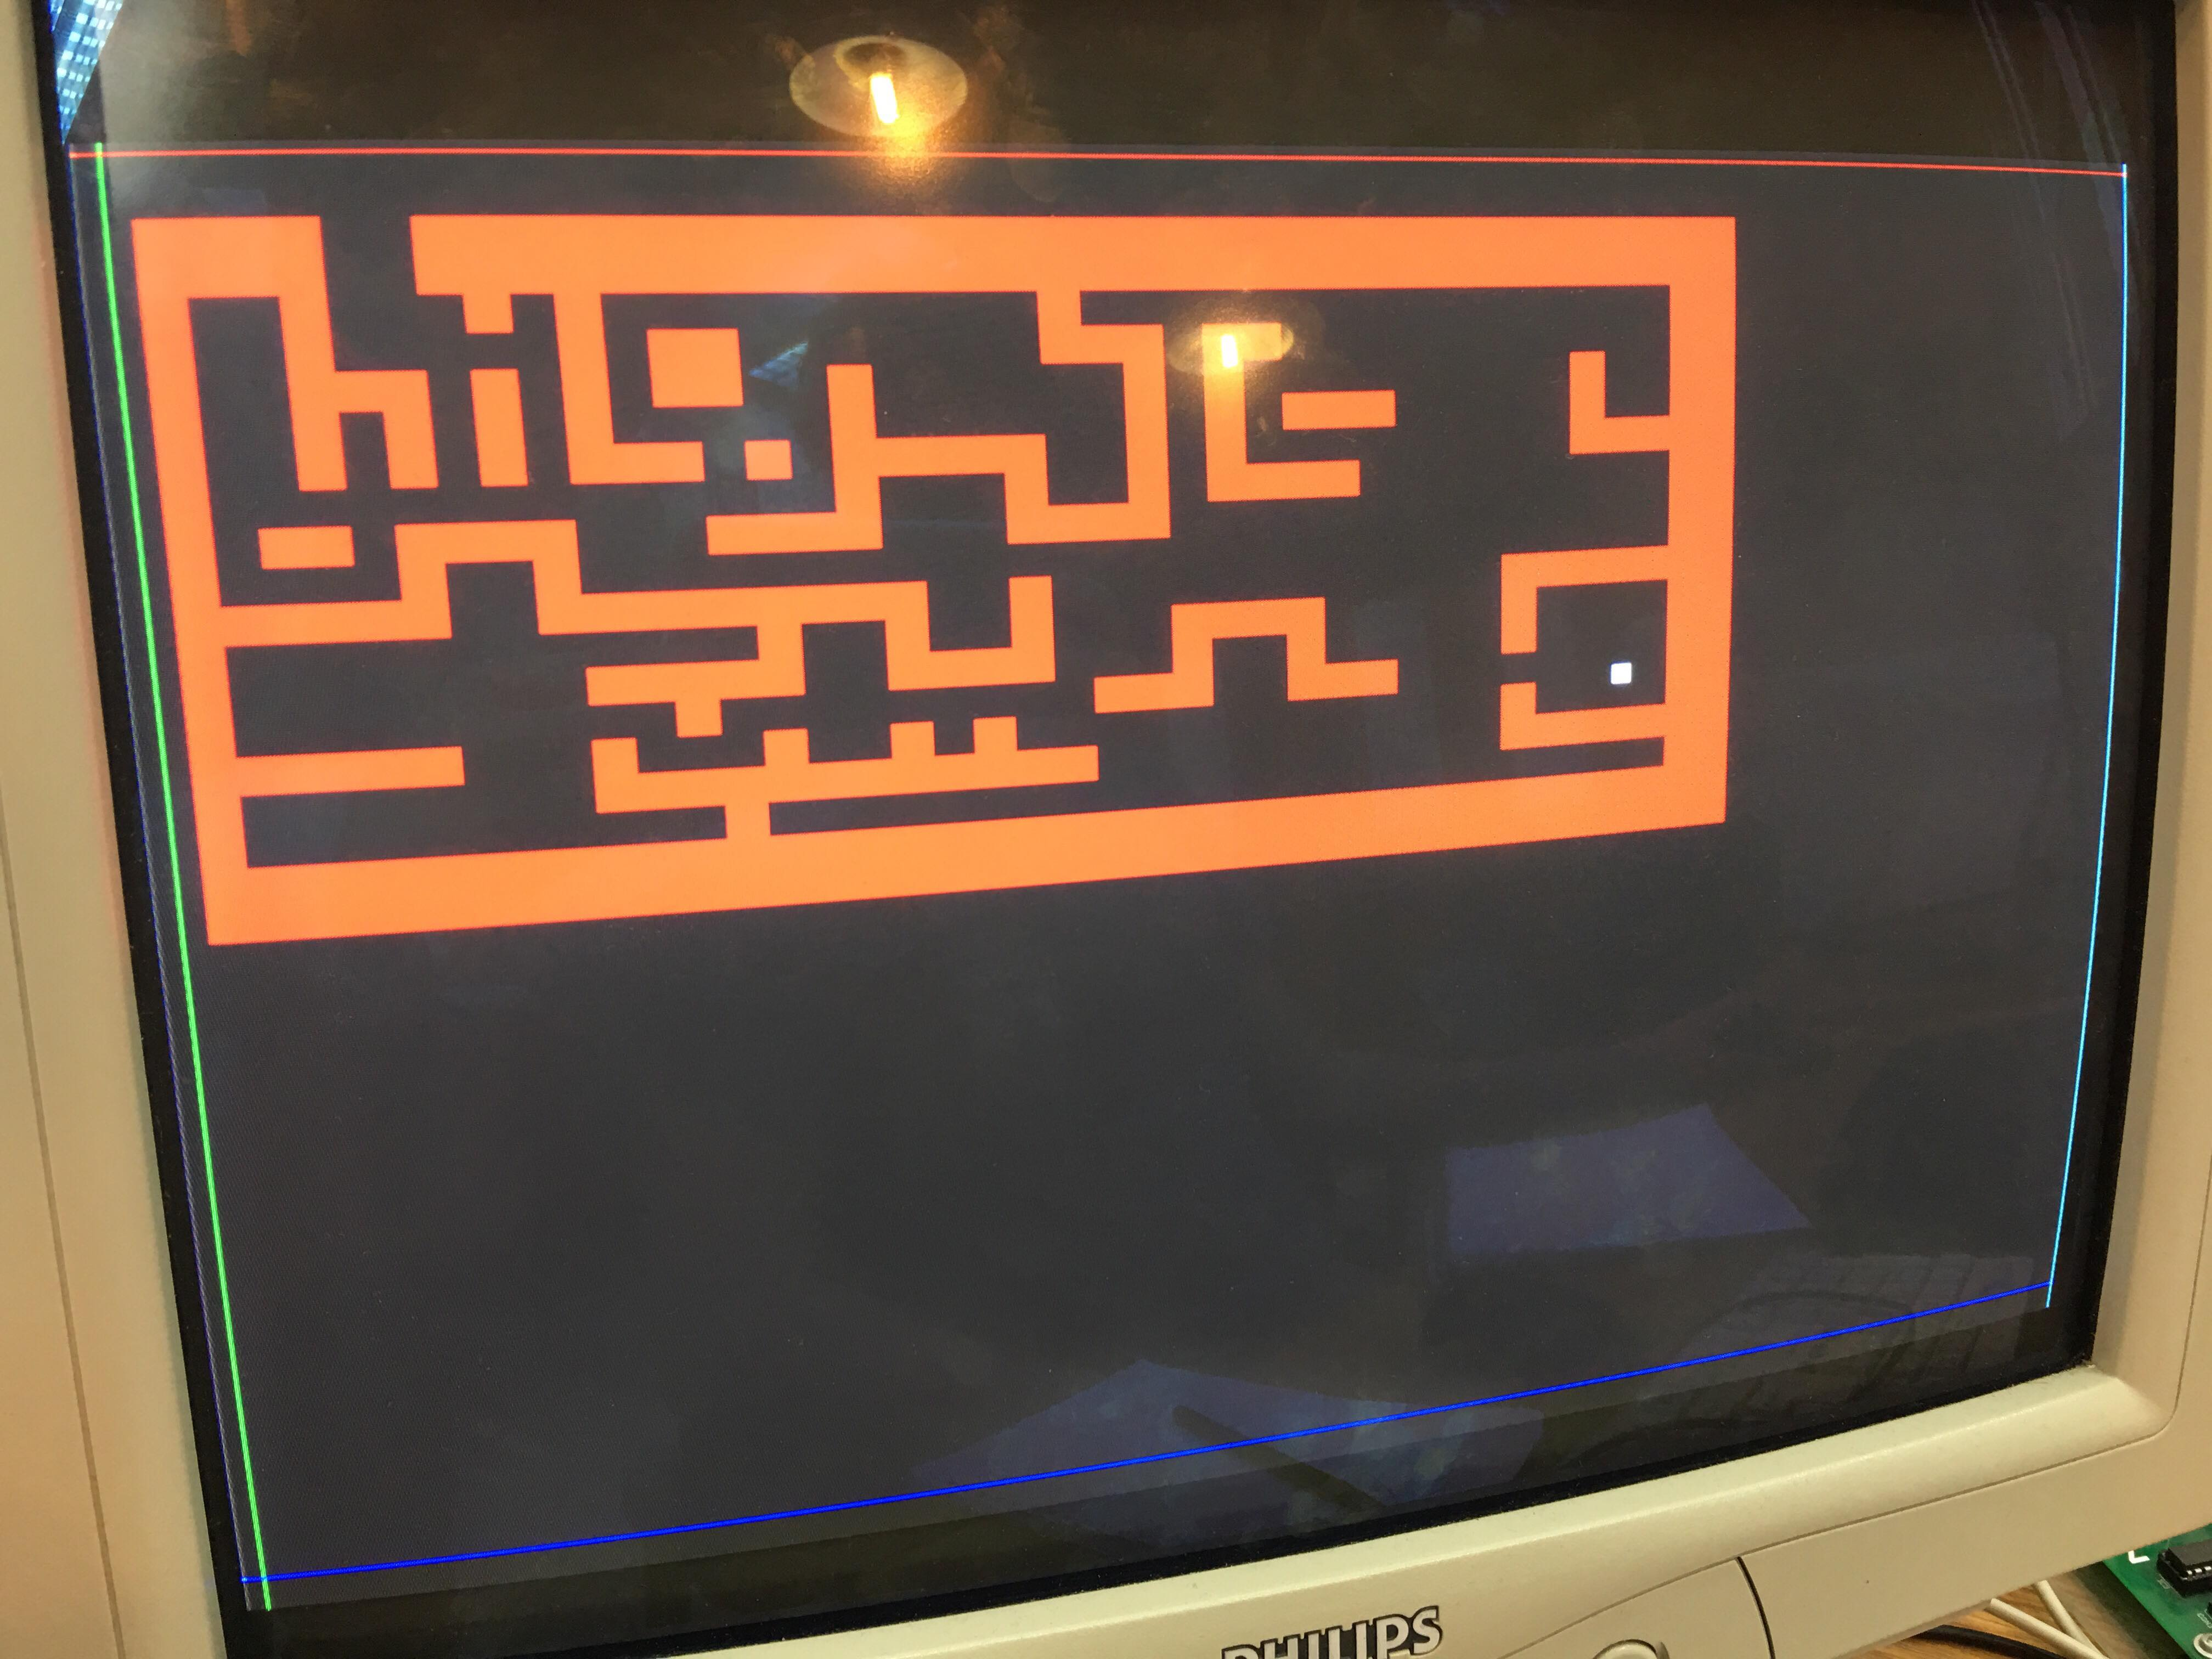
\includegraphics[scale=0.05]{start}
  \centering
\end{figure}

Gracz znajduje się na pozycji oznaczonej białym kursorem (kwadratem). Ściany oznaczone są kolorem pomarańczowym. Warto zauważyć też, że oznaczone zostały też krawędzie ekranu, za które nie może wyjechać kursor ponieważ przewyższają one rozdzielczość ekranu (widać je na zdjęciach ze względu na wymuszenie przez nas  oddalenia w opcjach monitora komputerowego).

\begin{figure}[H]
  \caption{Gra w akcji}
  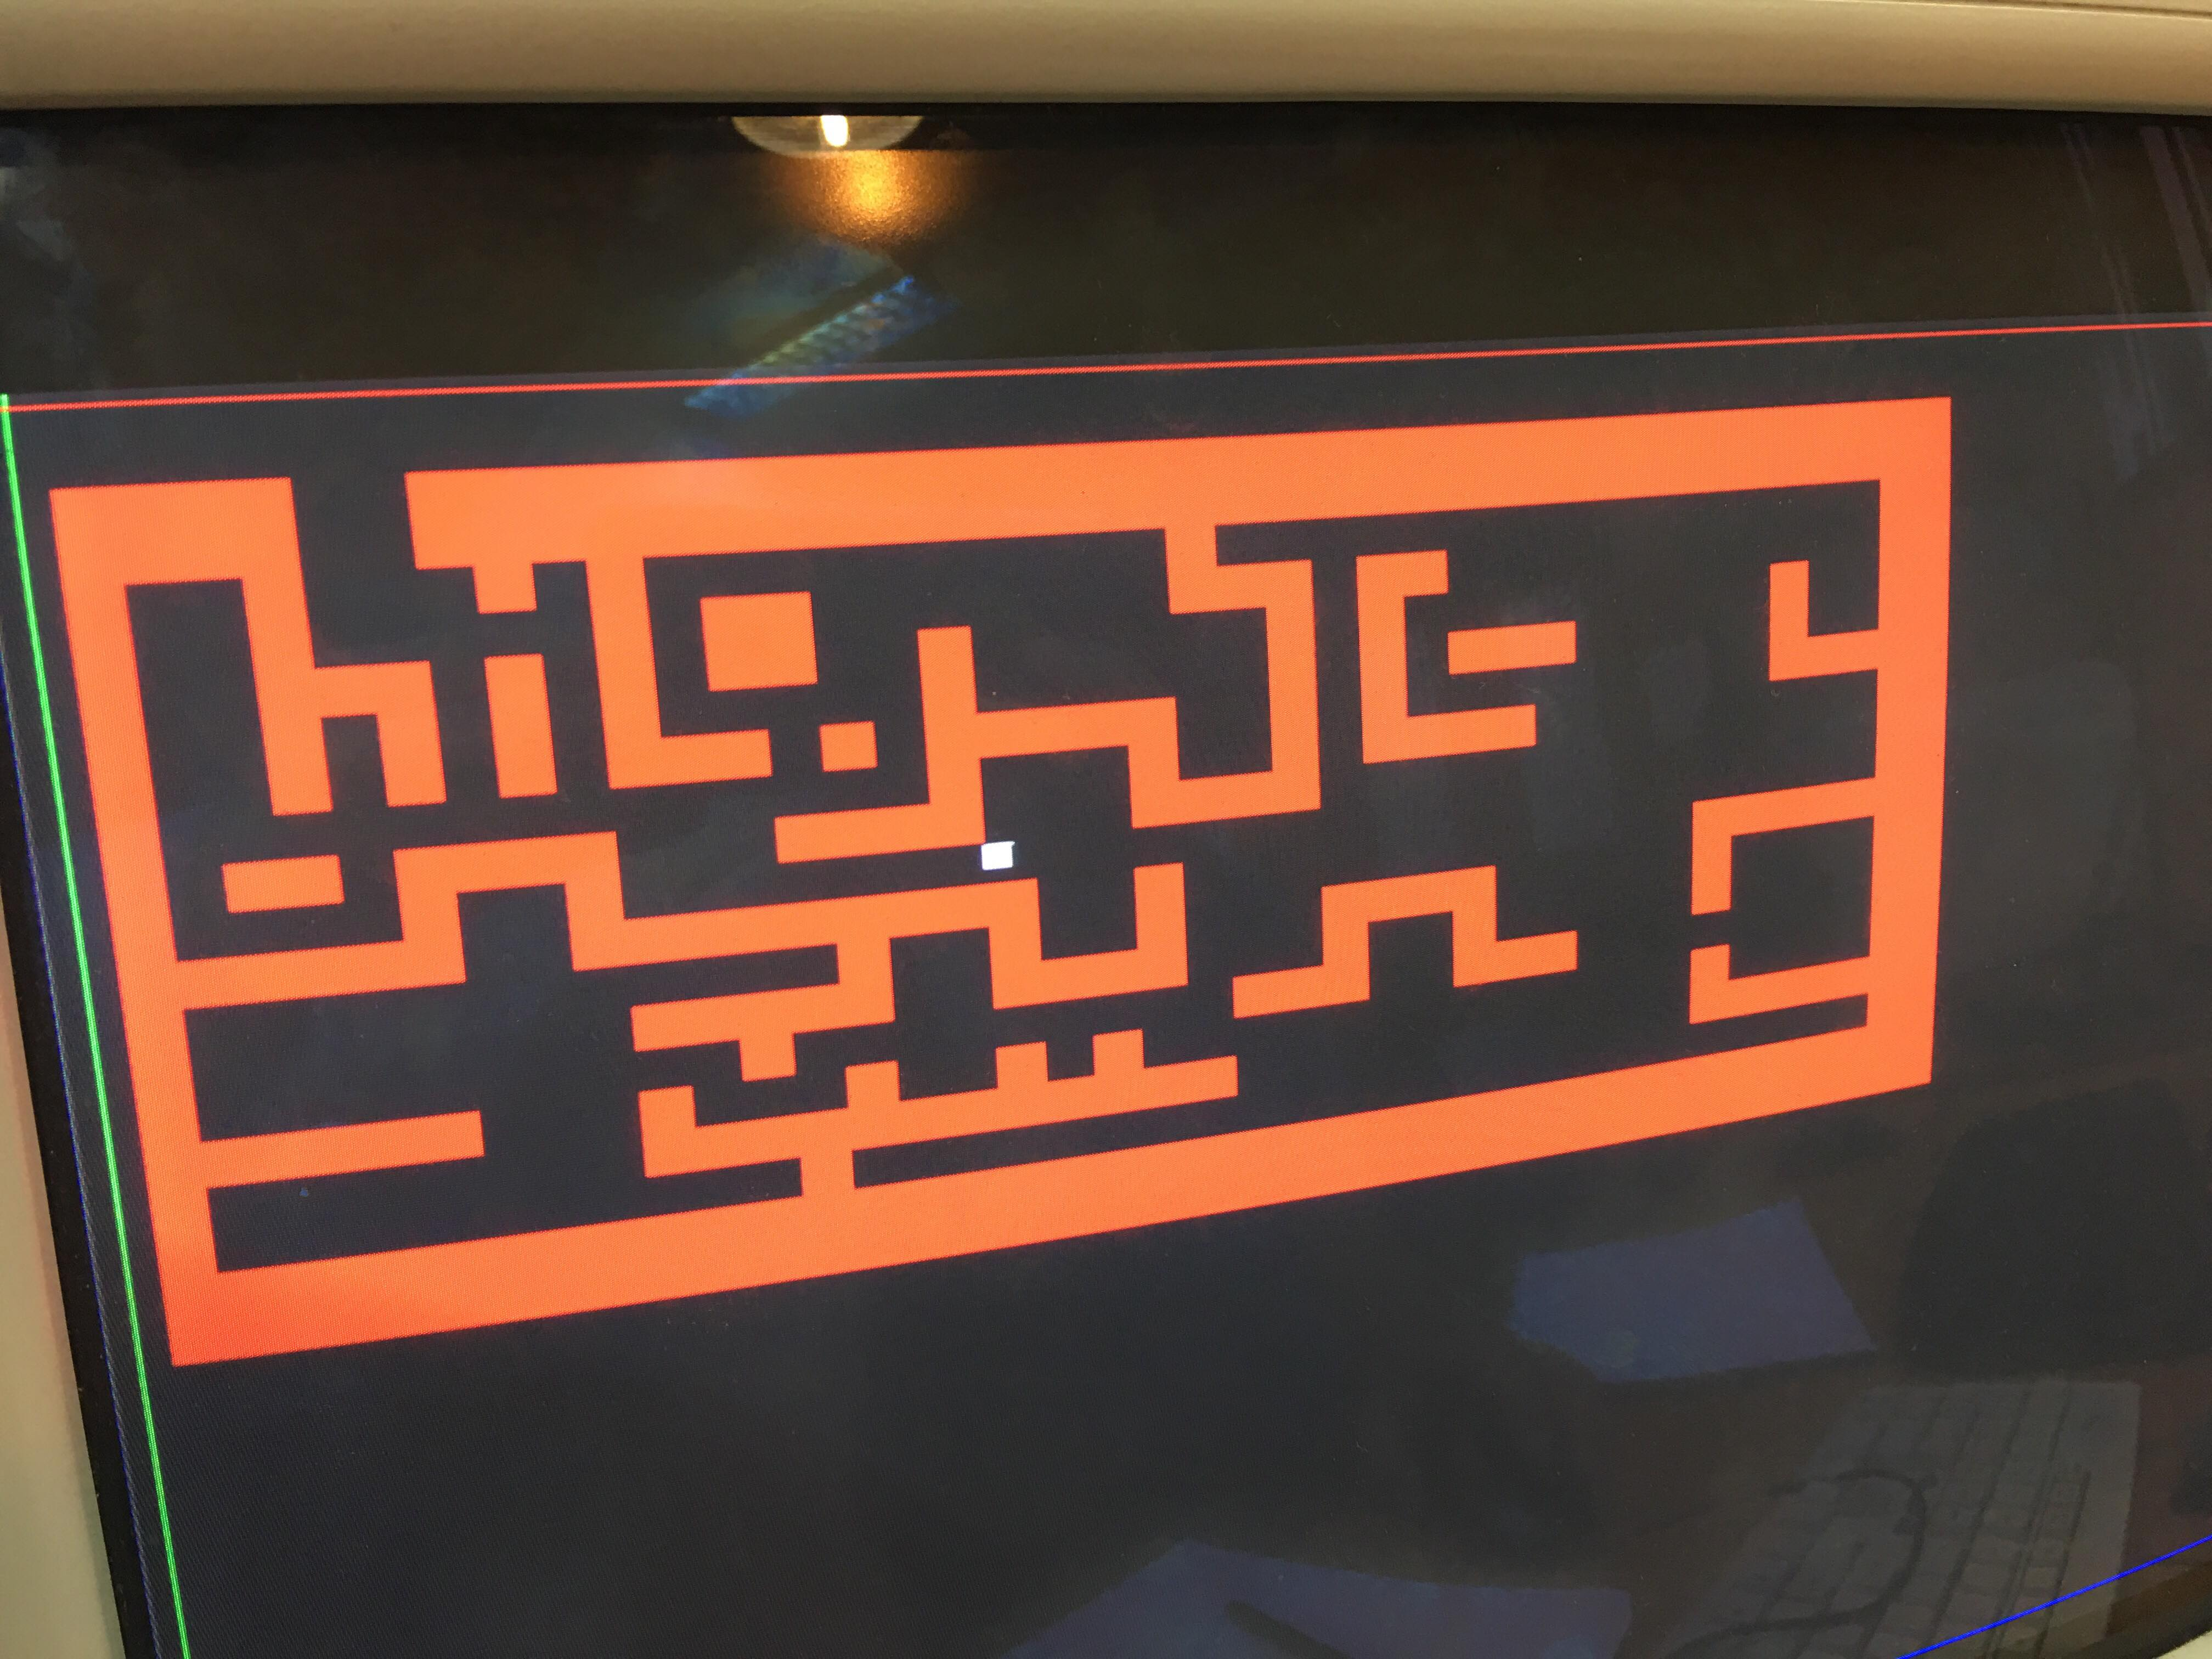
\includegraphics[scale=0.05]{gra1}
  \centering
\end{figure}

Gdy gracz dotknie ściany, oznacza to przegraną. Ekran wtedy usuwa labirynt z ekranu, pozwalając graczowi na swobodne poruszanie się po mapie i uniemożliwiając zapamiętanie drogi przy następnej próbie (utrudnienie rozgrywki).

\begin{figure}[H]
  \caption{Przegrana}
  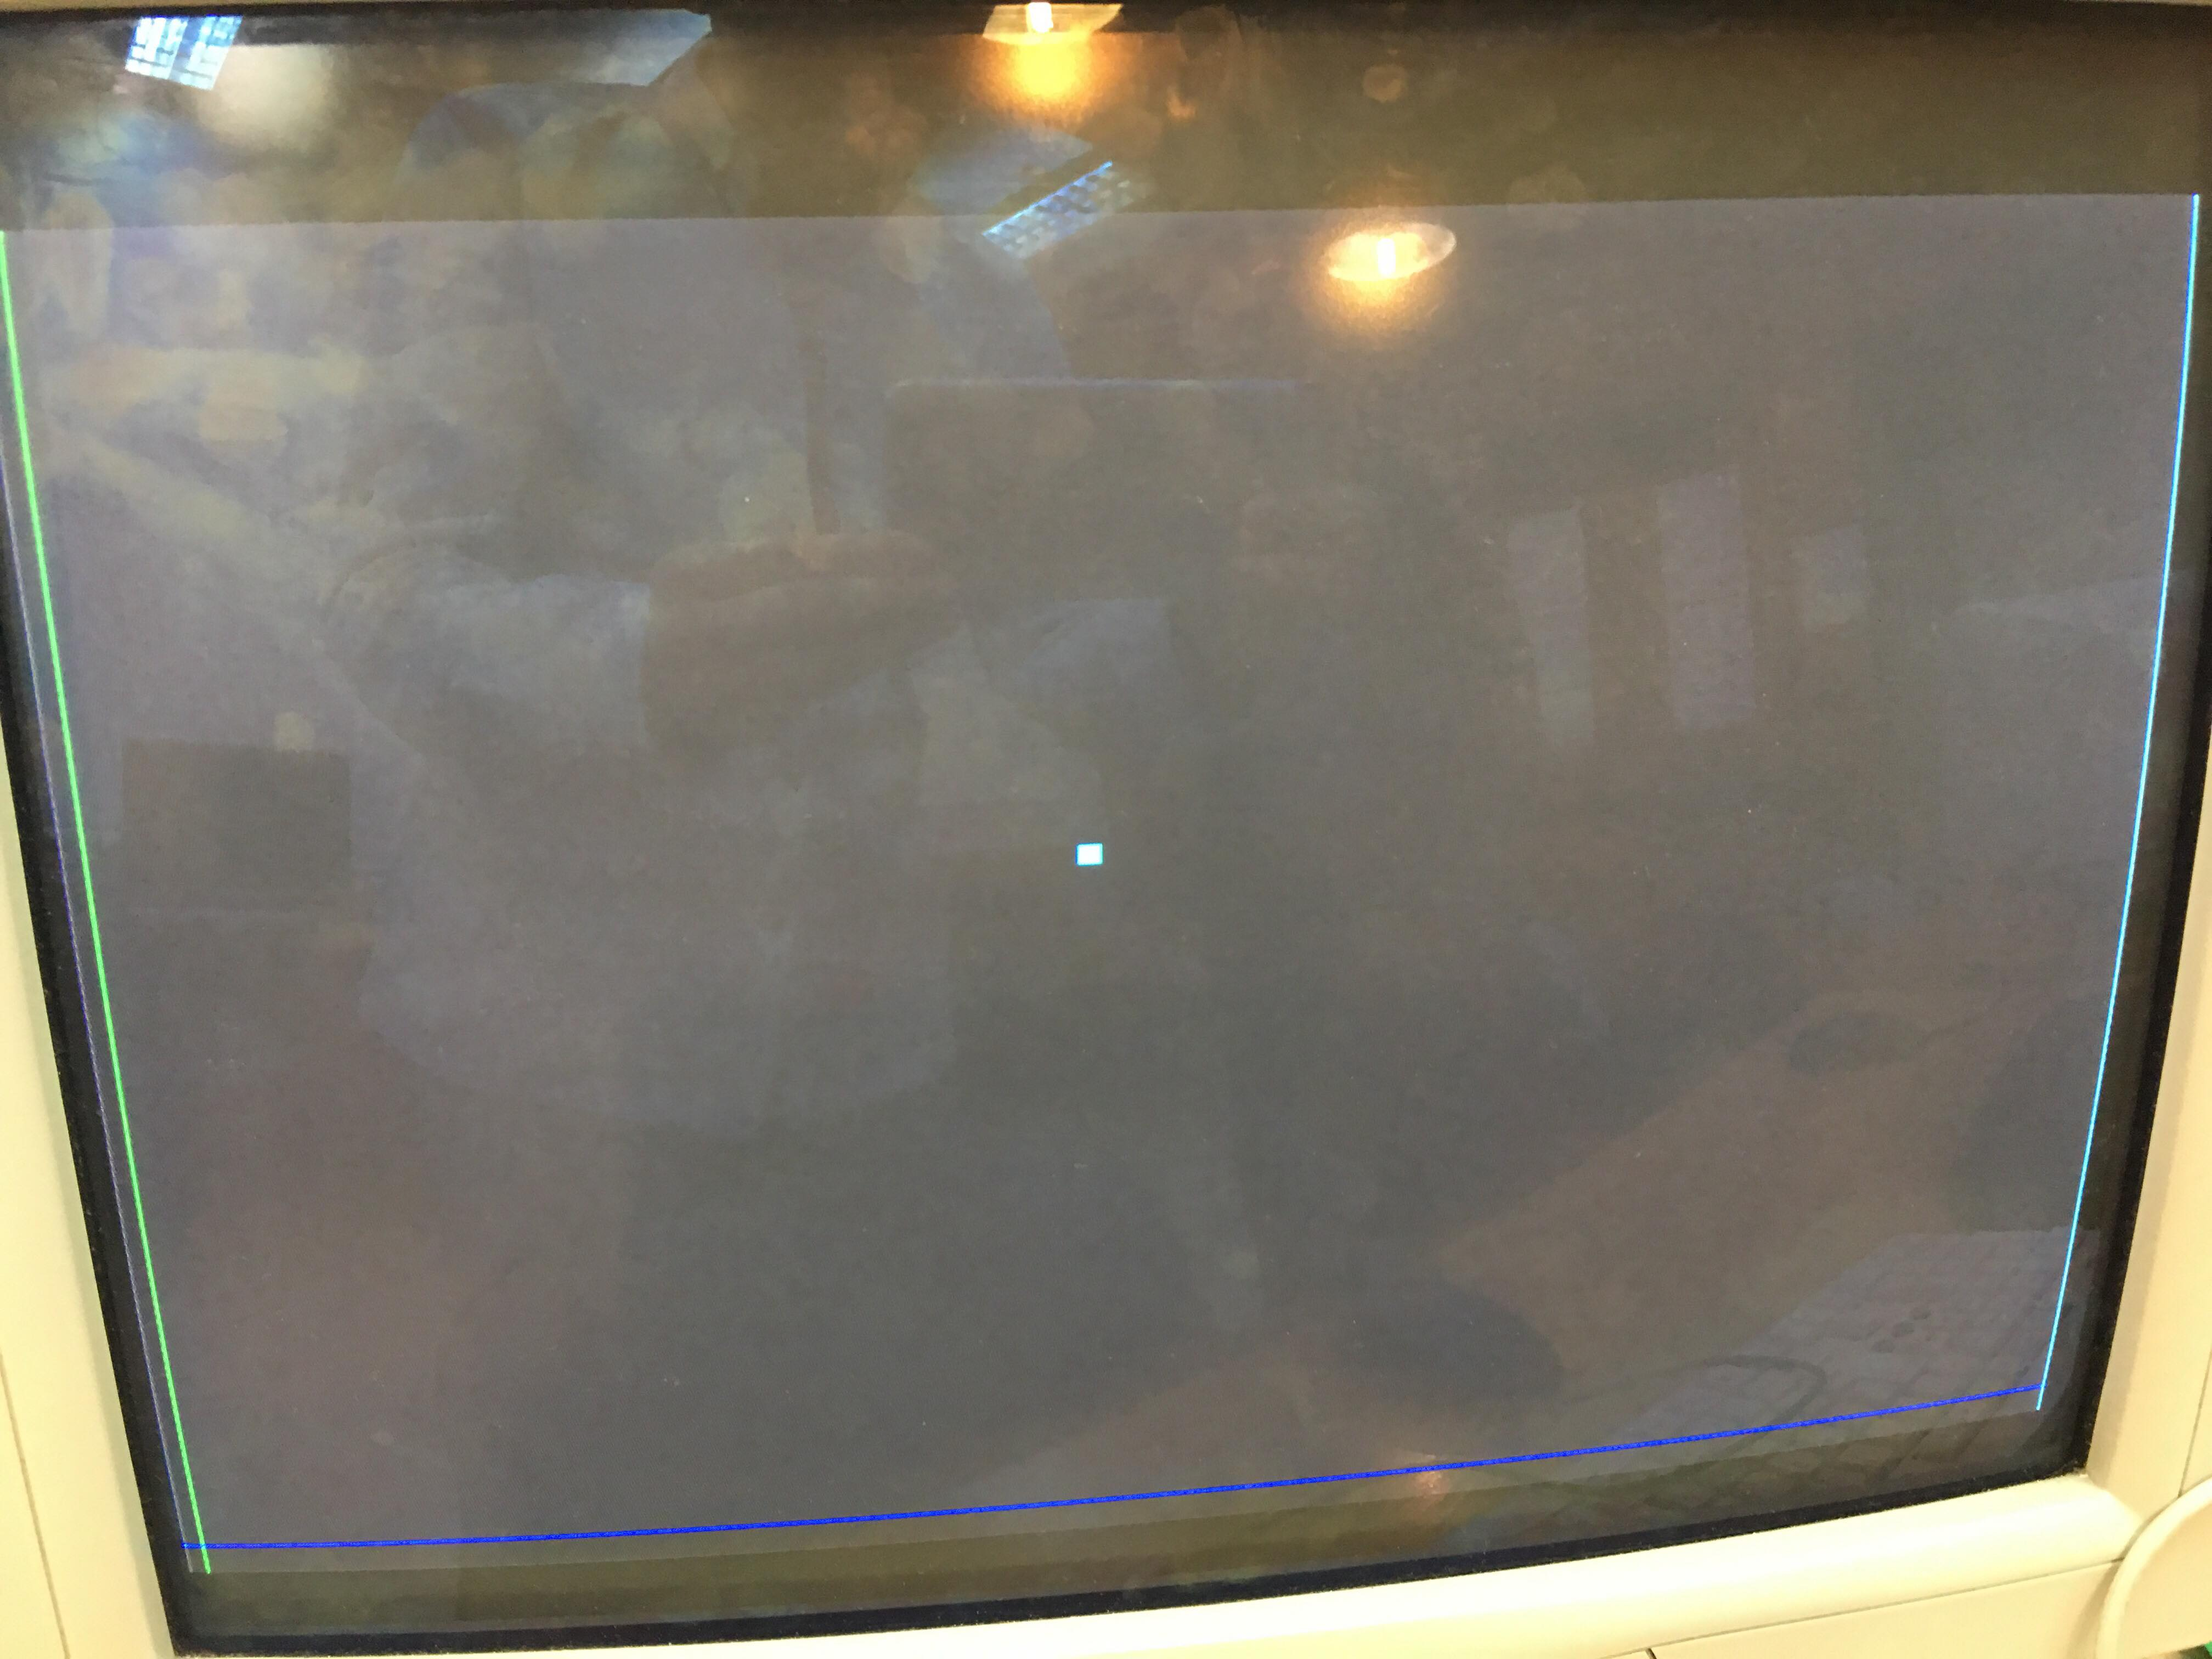
\includegraphics[scale=0.05]{przegrana}
  \centering
\end{figure}

Używając myszki gracz musi wymijać ściany i dotrzeć do wyjścia. W niektórych miejscach przejścia są odpowiednio węższe a do mety może prowadzić kilka dróg. Są jednak też drogi ślepe.

\begin{figure}[H]
  \caption{Gra w akcji}
  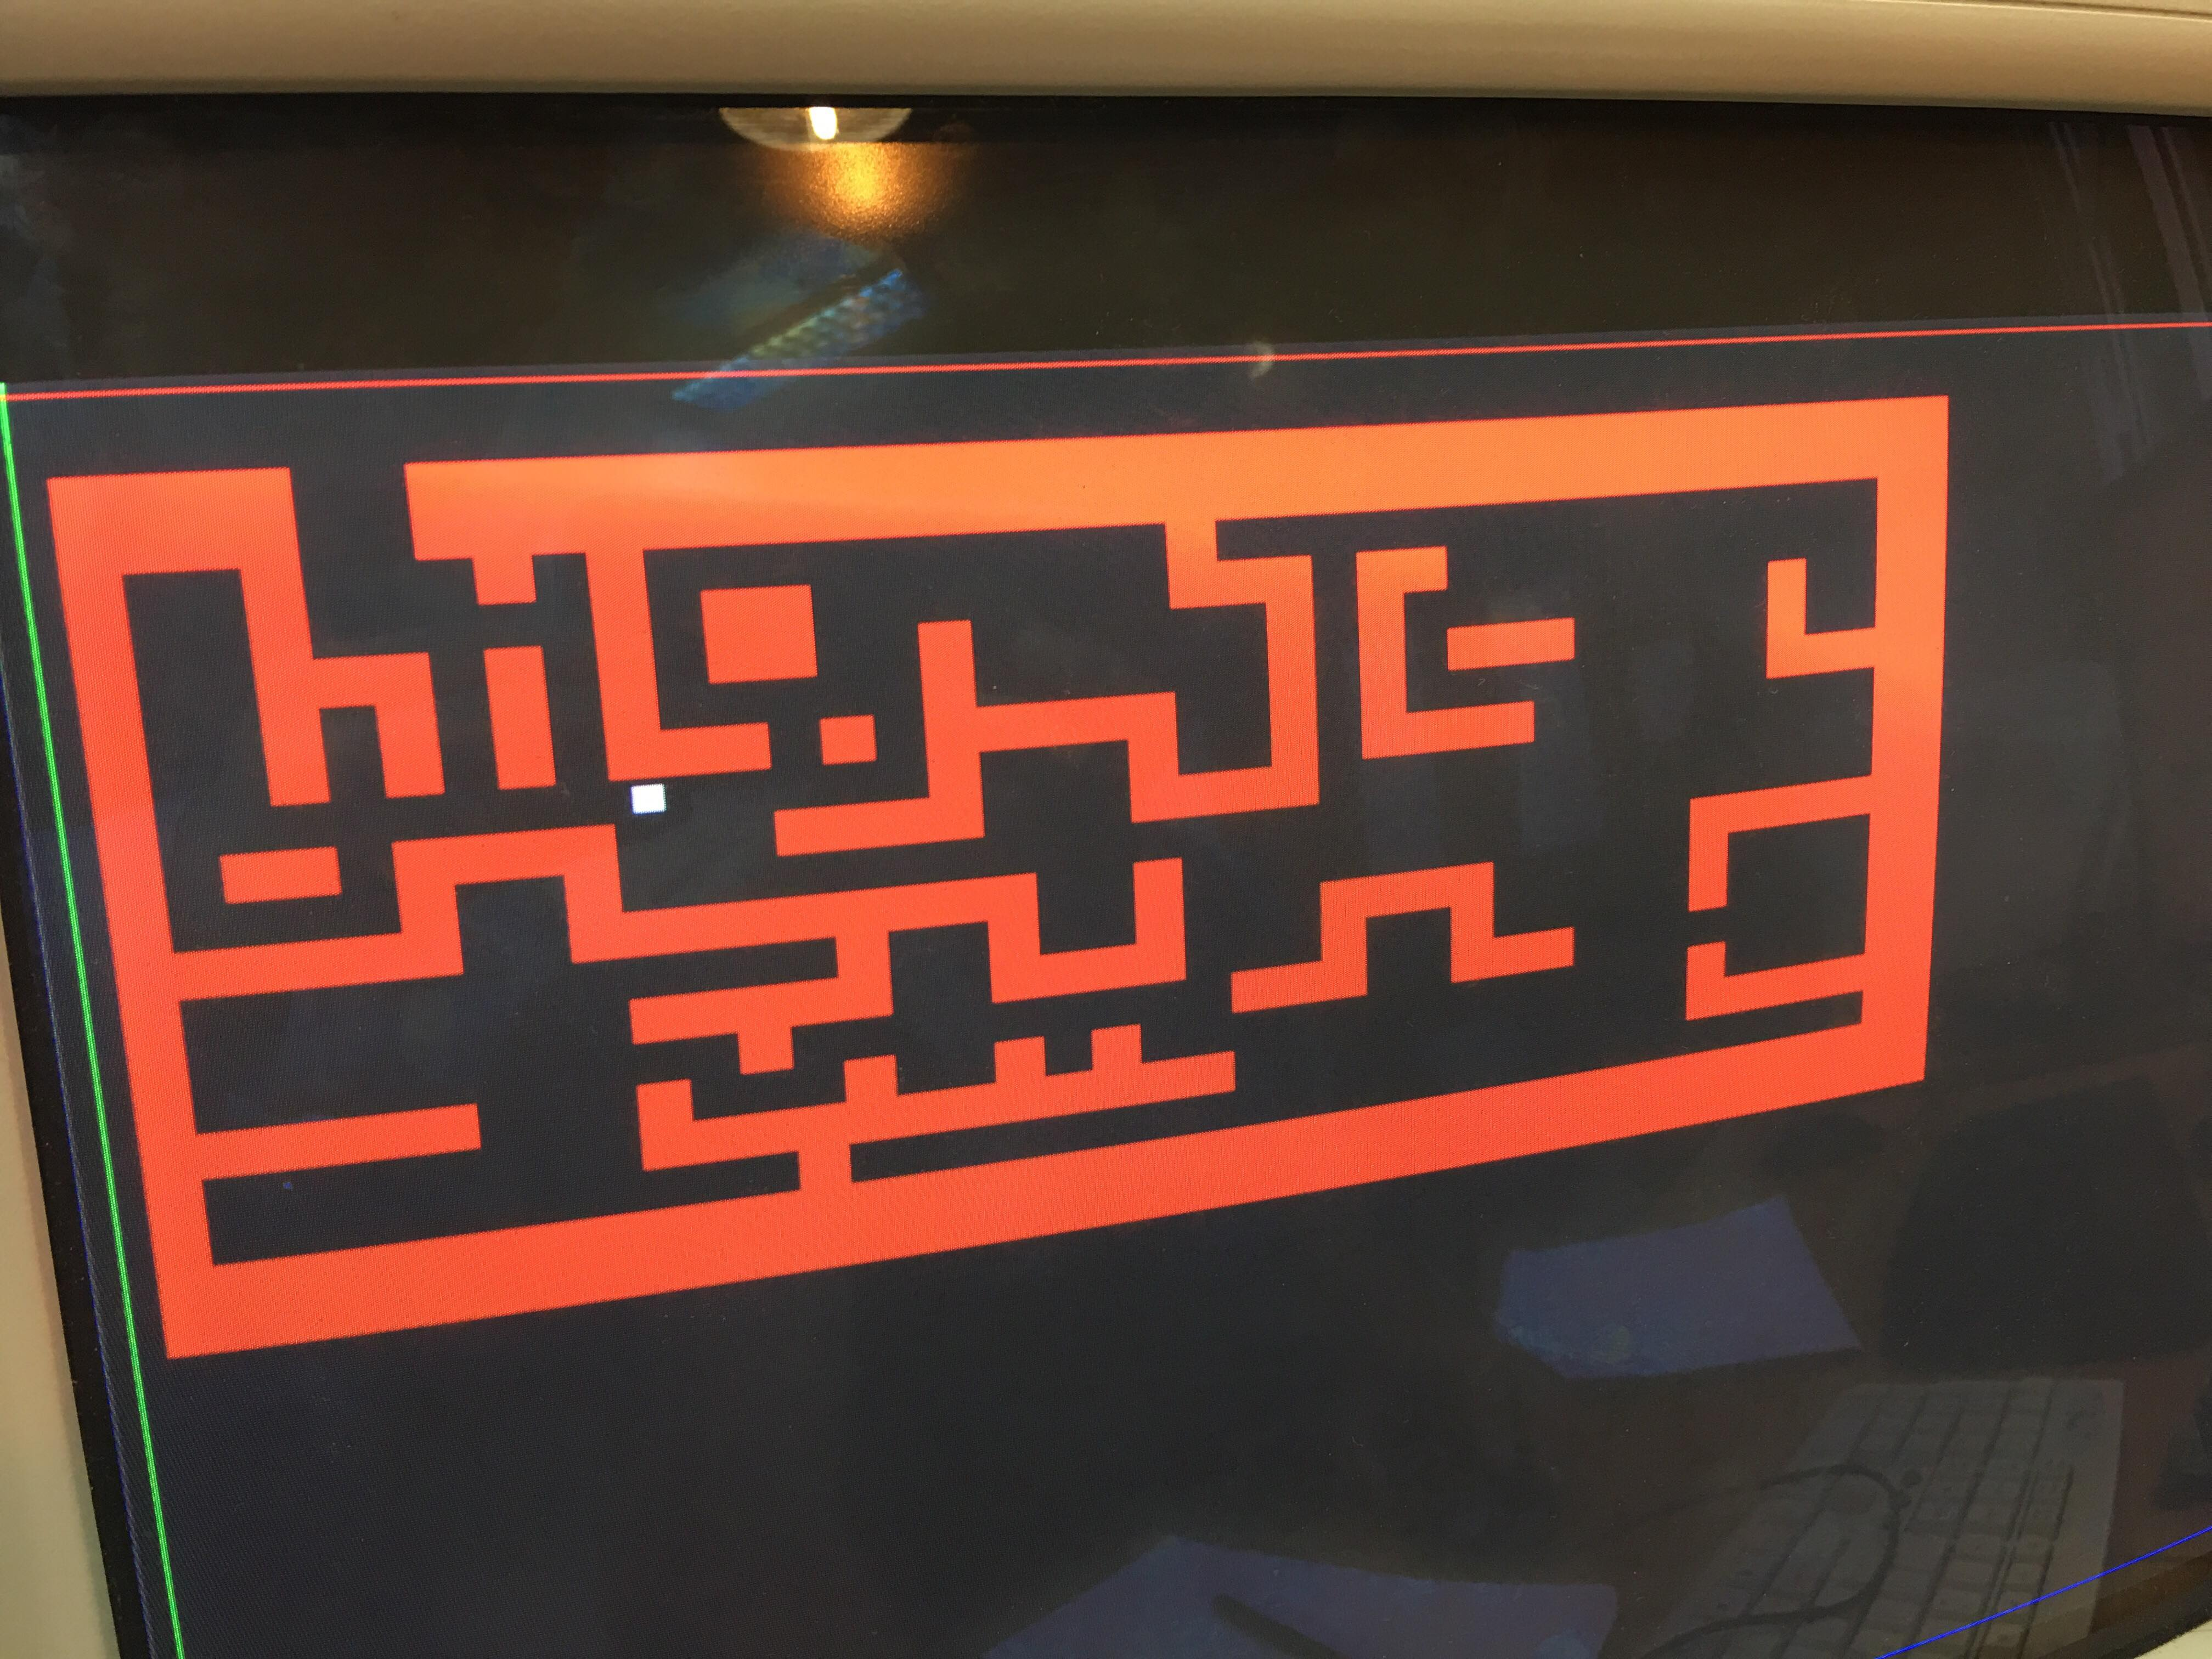
\includegraphics[scale=0.05]{gra2}
  \centering
\end{figure}

Gra kończy się gdy gracz dotknie kursorem myszy krawędzi górnej ekranu.

%%%%%%%%%%%%%%%%%%%%%%%%%%%%%%%%%%%%%%%%%%%%%%%%%%%%%%%%%%%%%%%%%%%%%%%%%%%%%%%%%%%%%%%%%%%%%%%%%%%%%%%%%%%%%%%%%%%%%%%
\section{Podsumowanie}

Na pierwszych zajęciach po wybraniu tematu i początkowych założeń projektowych rozpoczęliśmy pracę nad komunikacją między monitorem a płytką. W ciągu dwóch pierwszych zajęć udało się nam wyświetlić na prawidłowej rozdzielczości i odświeżaniu monitora (800x600 72Hz) pierwsze piksele. Na trzecich zajęciach udało się nam skomunikować myszkę i monitor, udało się uzyskać kwadrat na ekranie którym mogliśmy już sterować. Na kolejnych zajęciach zajęliśmy się utworzeniem modułu który miał przechowywać planszę gry w pamięci, udało się też utworzyć ograniczenie ruchu myszki tylko do widocznej części monitora. Piąte i szóste zajęcia pracowaliśmy nad systemem kolizji ze ścianami, opracowaniem wyglądu planszy, systemu przegranej, wygranej oraz nad innymi, pomniejszymi poprawkami w kodzie.

Trudnością szczególnie na początku było przypomnienie sobie schematów działania z układami cyfrowymi z poprzedniej części tego kursu. Każdy z etapów wyżej wymienionych różnił się od siebie, więc praktycznie na każdych zajęciach poruszaliśmy nowe zagadnienia. Bardzo przydatna okazała się dokumentacja dotycząca VGA i PS/2 która pozwoliła zrozumieć nasze zadania, oraz pomyślnie je wykonać. Co ciekawe, zrozumienie sposobu implementacji bloku pamięci do programu pomogło nam również zrozumieć działanie pamięci w dzisiejszych systemach operacyjnych.

Projekt ten pozwolił nam zrozumieć jak działają urządzenia których użyliśmy. Monitory wyposażone w złącze VGA czy myszki korzystające z portu PS/2 wciąż są dostępne i stanowią sporą część rynku mimo, że są powoli wypierane, kolejno: VGA przez HDMI, a PS/2 przez USB. Projektowa część tego kursu okazała się też ciekawsza niż poprzednia, laboratoryjna część kursu (mimo, że tamta dała nam niezbędną wiedzę), ze względu na to, że w tym semestrze uczestniczyliśmy aktywnie w stworzeniu czegoś większego i własnego. Według nas mieliśmy po prostu znacznie większy wpływ na to co napiszemy, zarówno od strony implementacji jak i samego wymyślenia wszystkich funkcjonalności, których implementacji będziemy chcieli się podjąć.

%%%%%%%%%%%%%%%%%%%%%%%%%%%%%%%%%%%%%%%%%%%%%%%%%%%%%%%%%%%%%%%%%%%%%%%%%%%%%%%%%%%%%%%%%%%%%%%%%%%%%%%%%%%%%%%%%%%%%%%
\section{Spis literatury}
\begin{itemize}
\item \url{https://www.xilinx.com/support/documentation/boards_and_kits/ug230.pdf}
\item \url{http://www.mikekohn.net/micro/fpga_vga.php}
\item \url{http://www.tinyvga.com/vga-timing/800x600@72Hz}
\item \url{http://www.zsk.ict.pwr.wroc.pl/zsk_ftp/fpga/#_Toc479592712}

\end{itemize}


\end{document}